\documentclass[UTF8,11pt,a4paper,fontset=none]{ctexart}
\usepackage{gbstyle}
\setCJKmainfont{Noto Serif CJK SC}
\setCJKsansfont{Noto Sans CJK SC}
\setCJKmonofont{Noto Sans CJK SC}
\renewcommand{\figurename}{图}
\renewcommand{\tablename}{表}
\begin{document}
\begin{center}
{\sffamily\bfseries\LARGE GraphBudget}\\[5pt]
{\sffamily\Large SGLang 确定性解码性能优化}\\[8pt]
{\small\color{GBGray}技术报告 \quad | \quad 2026 年 10 月 28 日}
\end{center}
\vspace{3mm}
\begin{center}
\begin{tabular}{ccc}
\GBmetric{+72.4\%}{吞吐配对提升中位数} &
\GBmetric{5}{组交错 A/B} &
\GBmetric{595}{项 GEMM 与重排检查}
\end{tabular}
\end{center}
\vspace{2mm}
\noindent\textbf{摘要。}
GraphBudget 面向 SGLang 确定性解码（Deterministic Decode）的性能问题，研究可选的 BF16 Small-$M$ GEMM 执行优化。项目参考 SGLang PR \#42145 中的分块几何方案，在固定 SGLang v0.5.9 Triton 路径上完成适配、原生回退、正确性与请求级性能验证。在 RTX 5070 Laptop、Qwen2.5-0.5B-Instruct BF16 及限定负载下，五组交错配对的有效输出吞吐提升中位数为 \textbf{72.4\%}。本结果只属于明确的模型、硬件与执行配置，不代表跨模型、跨框架或生产服务的通用收益。原始 CUDA Graph 成本策略与 Decode Metadata 候选没有确立稳定的增量收益，相关实验结果单独保留。

\Needspace{7\baselineskip}\section{问题与技术目标}
在推理 Decode 阶段，部分 BF16 矩阵乘的输出行数 $M$ 很小，传统较大的矩阵 Tile 可能不匹配实际工作负载。当前实验版本的确定性 SGLang 使用 persistent Triton GEMM。研究目标是在不改变既有 FP32 累加和融合 Bias 数值语义、也不放宽原生执行安全条件的前提下，验证小 $M$ 分块方案是否能改善真实请求完成效率。

本项目的可量化性能结果来自 \textbf{Small-$M$ GEMM 路径适配}。其 Tile 思路来源于 bill-h-lin 的 \href{https://github.com/sgl-project/sglang/pull/42145}{SGLang PR \#42145}；本项目完成的是对固定执行版本的适配、路径接入、验证与测量，不将其称为自创 GEMM 算法，也不声称获得上游合并。



\Needspace{7\baselineskip}\section{实现范围与数值契约}
性能分支为 \texttt{\_matmul\_persistent\_triton} 引入可关闭的候选路径。只有显式启用开关、输入为 BF16、$0<M\le16$、$K\bmod64=0$、$N\bmod128=0$ 且相关内层 Stride 满足条件时，才选择 $B_M=16$、$B_N=64$、$B_K=128$、四个 Warp、一个程序处理一个输出 Tile 的方案；其余调用沿用原生实现。

候选和基线共享既有 persistent Triton GEMM 计算结构，保留 FP32 累加与 fused-bias 的计算次序，避免用更快但不满足当前确定性契约的路径替代。改动不会引入在线 CUDA Graph 重新捕获、新的请求准入调度器或 GPU 到 CPU 的逐步同步读取。原有图执行与安全判断仍由 SGLang 负责。

\begin{figure}[H]
\centering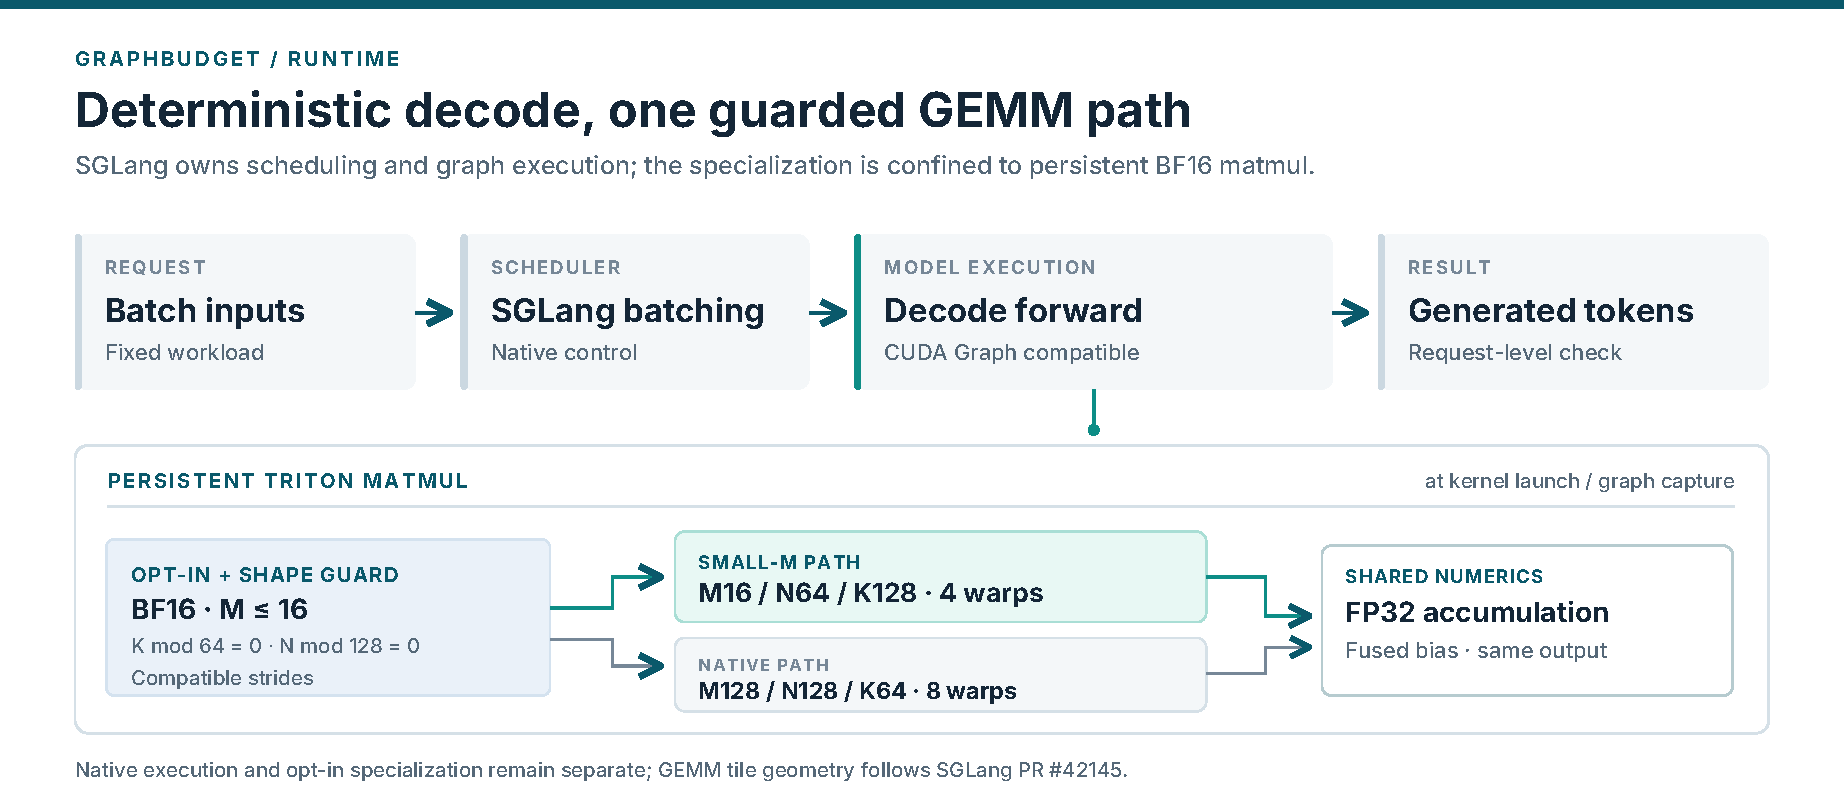
\includegraphics[width=\textwidth]{../figures/decode_architecture.pdf}
\caption{推理执行边界与 Small-$M$ 路径。Kernel 选择发生在实际 Launch 准备或 Graph Capture 阶段，已捕获的 CUDA Graph 在 Replay 时不会逐 Token 重新动态选路。}
\end{figure}

\Needspace{14\baselineskip}\section{实验环境与比较协议}
\begin{table}[H]\centering\small
\caption{固定版本与正式实验条件}
\begin{tabularx}{\textwidth}{@{}p{.27\textwidth}X@{}}\toprule
项目 & 条件 \\\midrule
运行环境 & SGLang v0.5.9（基线 SHA：\texttt{bbe9c7e...}），RTX 5070 Laptop，WSL \\
软件栈 & PyTorch 2.9.1+cu128，Triton 3.5.1，确定性 Triton \\
模型 & Qwen2.5-0.5B-Instruct，BF16，TP=1，贪心解码 \\
服务限制 & 最多 16 个正在执行的请求；Graph 捕获大小 $[1,2,4,8,12,16]$；关闭 Overlap \\
正式工作负载 & 每个实验臂 256 个固定请求，每个请求输出 128 Token \\
对照协议 & 五组独立服务进程交错配对：AB、BA、AB、BA、AB \\
核心指标 & 有效输出 Tokens/s；先计算每组相对变化，再取中位数 \\\bottomrule
\end{tabularx}
\end{table}

\begin{figure}[H]
\centering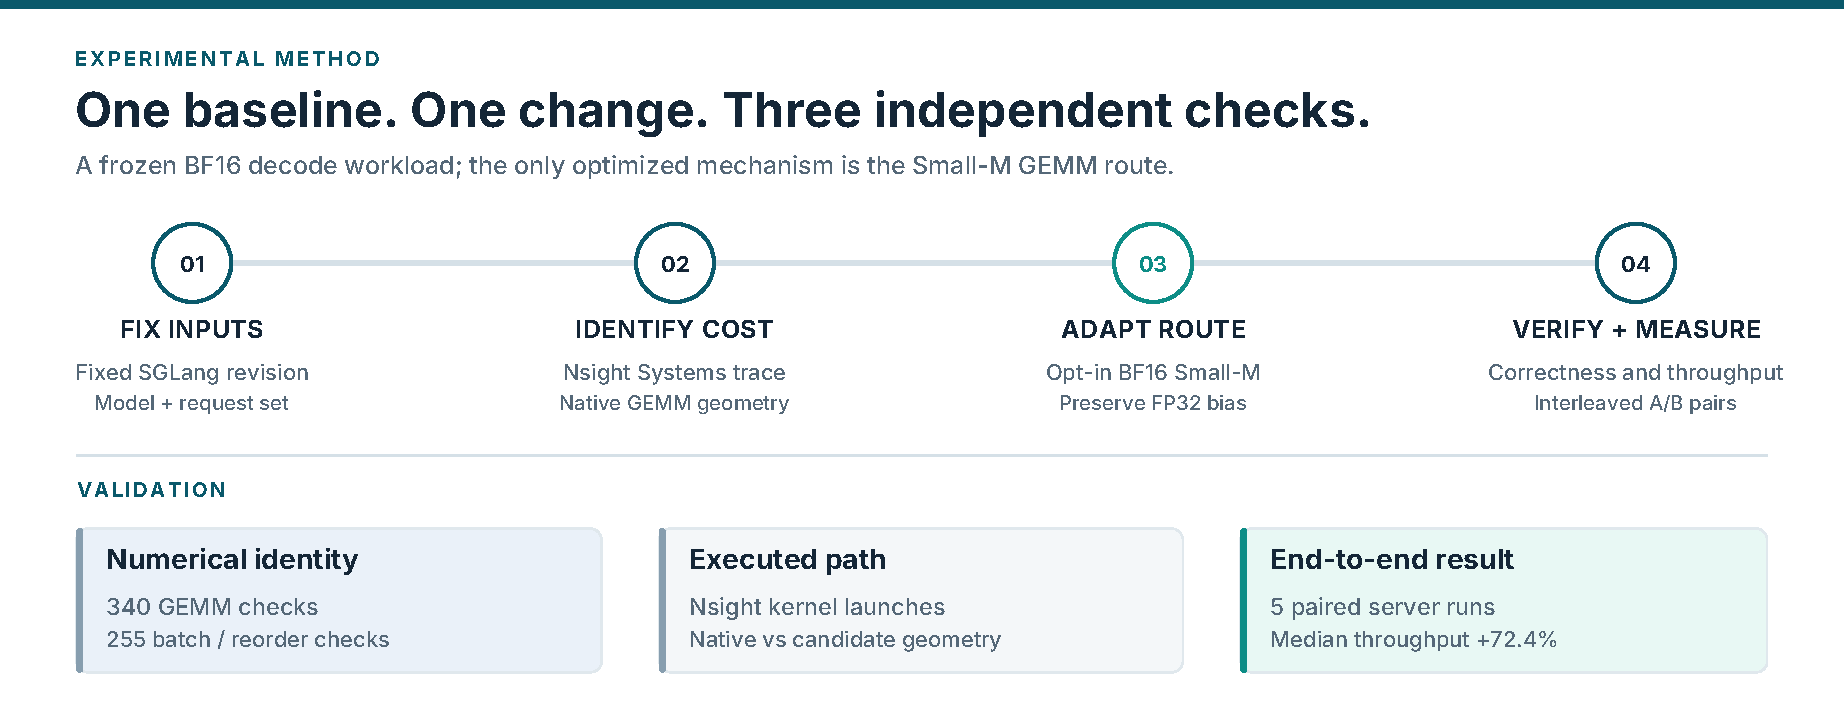
\includegraphics[width=\textwidth]{../figures/validation_workflow.pdf}
\caption{从固定环境、原生基线、性能剖析、候选适配，到数值验证和请求级 A/B。原预算策略与元数据优化作为独立消融结果记录。}
\end{figure}

\Needspace{7\baselineskip}\section{端到端吞吐结果}
\begin{table}[H]\centering\small
\caption{五组正式配对结果}
\begin{tabular}{@{}rrrr@{}}\toprule
组次 & 原生路径（Tokens/s） & 候选路径（Tokens/s） & 组内相对变化 \\\midrule
1 & 1,164.15 & 2,007.24 & +72.42\% \\
2 & 1,096.61 & 1,783.15 & +62.61\% \\
3 & 1,122.35 & 2,087.16 & +85.96\% \\
4 & 1,128.60 & 1,933.98 & +71.36\% \\
5 & 1,135.00 & 2,023.29 & +78.26\% \\\midrule
\multicolumn{3}{r}{配对相对变化中位数} & \textbf{+72.42\%}\\\bottomrule
\end{tabular}
\end{table}
\begin{figure}[H]
\centering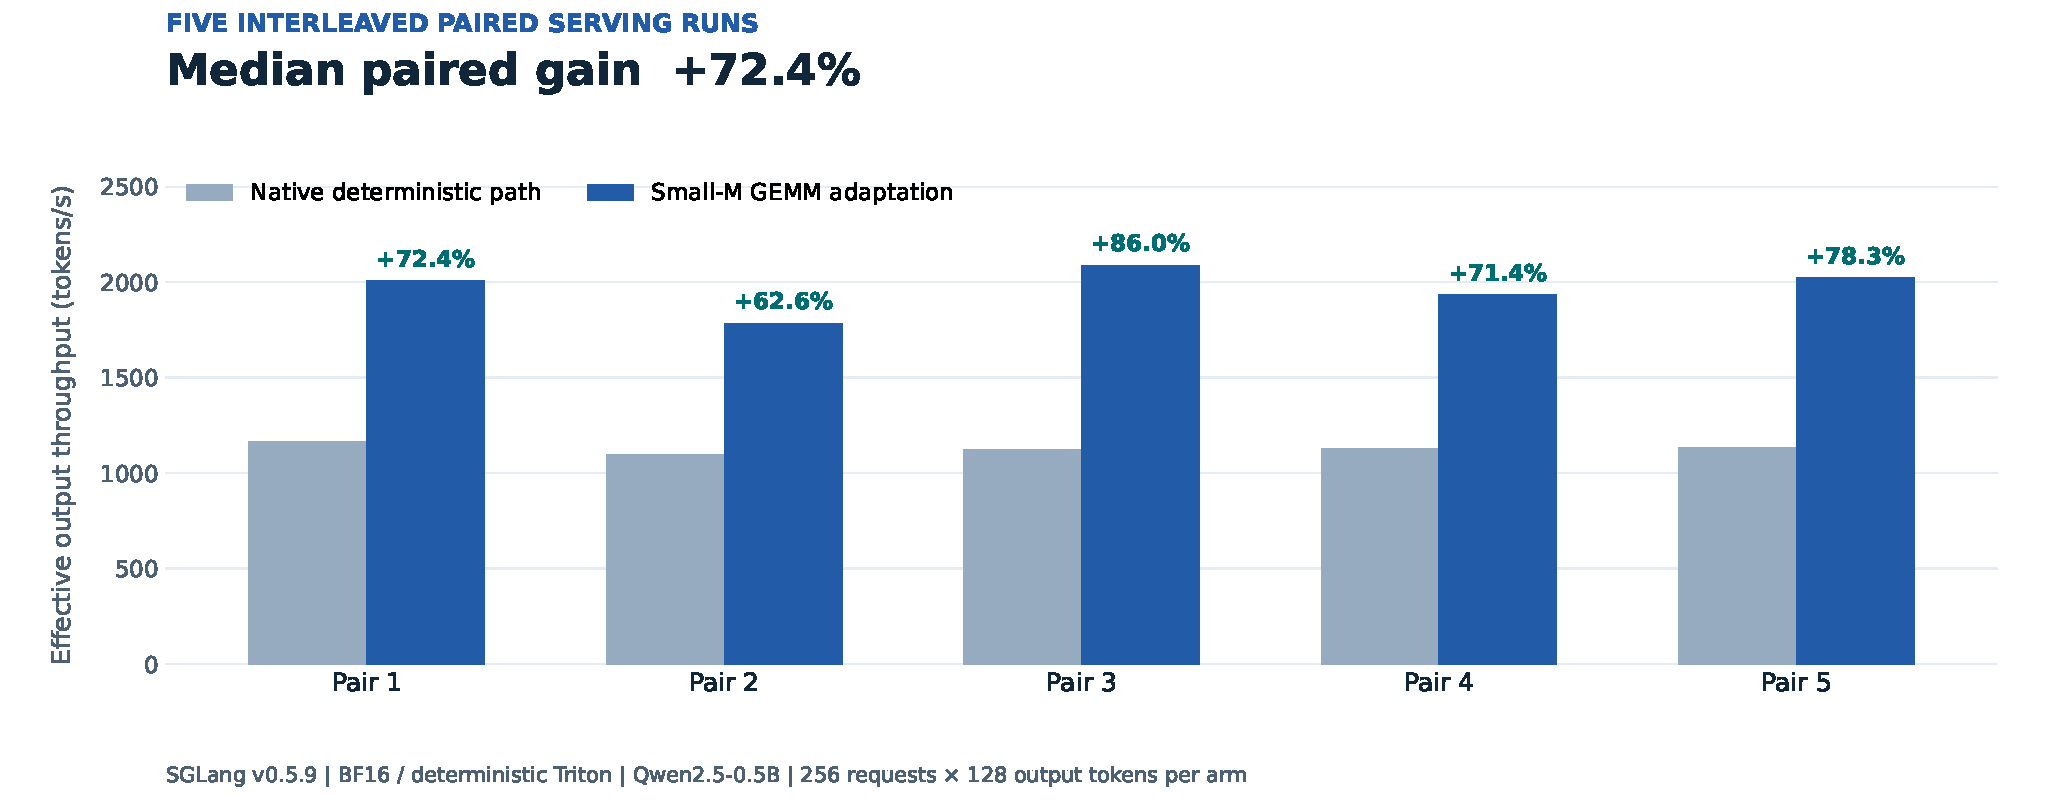
\includegraphics[width=\textwidth]{../figures/paired_throughput.pdf}
\caption{固定请求负载下的原生确定性路径与 Small-$M$ GEMM 候选。图中百分比表示各组配对相对变化，不能理解为与最新 SGLang 默认服务路径相比的通用加速。}
\end{figure}

五组主负载性能变化均为正；前、后 A/A 吞吐变化分别为 +7.9\% 与 +8.8\%。这两组 A/A 只能表示有限的噪声观测，不是置信区间。主负载的结果不能自动推广到开放到达率、不同模型或不同执行硬件。

\Needspace{7\baselineskip}\section{正确性与执行路径证据}
最终实际加载的 GEMM 源码通过 340 项数值检查，覆盖若干模型相关形状和 $M=1\ldots17$；其中 170 项具有独立精确 CPU 参考。全部 340 项与原生输出逐位一致。另外 255 项检查覆盖行重排、跨 Batch 复用和随机 Bias。正式请求输出在所测条件下逐 Token 一致。上述检查不代表任意形状、任意设备都已经验证。

Nsight Systems 记录中，两条执行臂均观察到 63 次 \texttt{cudaGraphLaunch}。原生臂的 6,305 次 \texttt{matmul\_kernel\_persistent} 活动均采用 256 Threads/Block；候选臂中 6,113 次采用 128 Threads/Block，另 192 次仍为 256。这表明目标 GEMM 的实际启动配置已经发生变化。Trace 用于路径诊断，正式吞吐结论使用未开启 Profiling 的独立请求测量。

\Needspace{7\baselineskip}\section{负结果、局限与下一步}
\begin{table}[H]\centering\small
\caption{单独成立的负结果与验证边界}\begin{tabularx}{\textwidth}{@{}p{.33\textwidth}X@{}}\toprule
实验方向 & 结论及其边界 \\\midrule
原 CUDA Graph 成本分派 & 相对公平静态设置没有稳定增量收益，继续采用原生分派。 \\
Metadata 预分配 & 两个对照区块分别为 +0.8\%、$-1.0$\%；没有建立稳定性能增益。 \\
Metadata Fusion & 分别为 $-3.4$\%、$-6.1$\%，不作为正向优化成果。 \\
Holdout 首 Token 延迟 & TTFT p50 配对变化方向不一致，中位数 +21.5\%（更差），不能宣称普遍降低延迟。 \\
显存与启动 & 未确立 VRAM 节省、KV 扩容或冷启动加速；启动实验存在文件系统差异。 \\
硬件性能计数器 & Nsight Compute 因 \texttt{ERR\_NVGPUCTRPERM} 未取得相关计数器；不推断实际 Occupancy 或带宽提升。 \\\bottomrule\end{tabularx}\end{table}

负结果否定的是具体成本策略和元数据候选的性能假设，\textbf{不否定已独立完成验证的 GEMM 适配结果}。后续应通过剖析确定新的高贡献性能热点，再决定是否进行独立优化。对跨模型、跨 GPU 的泛化验证应单独设计实验；目前没有相应结论。

\Needspace{7\baselineskip}\section{复现入口与来源}
\href{https://github.com/yu830/graph-budget-runtime}{公开仓库} 提供固定性能提交、SGLang Patch、机器可读的 A/B 汇总和运行环境说明。复现实验需严格对齐依赖版本、模型修订和请求参数；单组重跑不等于重现五组正式结果。
\begin{enumerate}[leftmargin=1.6em,itemsep=.18em]
\item \href{https://github.com/sgl-project/sglang/pull/42145}{bill-h-lin，SGLang PR \#42145}：Small-$M$ BF16 GEMM 的 Tile 思路与来源。
\item \href{https://github.com/yu830/graph-budget-runtime/blob/1f1984147608ee6c5dd8b3423e6f41877aaadeb4/docs/PERFORMANCE_RESULTS_20261027.md}{GraphBudget 原始性能记录}：固定条件、正式配对、消融和限制。
\item \href{https://github.com/yu830/graph-budget-runtime/blob/1f1984147608ee6c5dd8b3423e6f41877aaadeb4/src/graphbudget/patches/sglang-v0.5.9.patch}{SGLang Runtime 集成补丁}：路径门控、数值契约和观测点。
\item \href{https://github.com/yu830/graph-budget-runtime/blob/1f1984147608ee6c5dd8b3423e6f41877aaadeb4/THIRD_PARTY_NOTICES.md}{第三方许可与归属声明}。
\end{enumerate}
\end{document}
